\section{Beyond Grids: Exploring Elastic Input Sampling for Vision Transformers}
\label{sec:beyond}

\subsection{Motivation}
\label{sec:motivation-beyond}

As described in Section~\ref{sec:prelim-pos-enc}, a standard ViT relies on learnable positional embeddings indexed by grid position. This design choice is valid in standard benchmarks where every image is processed by the same fixed (most commonly) $14\times14$ grid of $16\times16$ patches, but it creates a fundamental brittleness in any deployment where the patch positions or sizes deviate from those seen during training. In real-world settings, a PTZ camera may not snap to discrete zoom levels, and a UAV may fly at an altitude that does not correspond to any training configuration. More importantly, an active vision system may benefit from being able to select a glimpse at a position not aligned to the standard patch grid. This publication asks, as an empirical question, how fragile standard ViTs are under such conditions, and what architectural and training changes are needed to make them robust.

It thereby investigates Hypothesis~\ref{hyp:beyond}: a vision transformer can be made resilient to input patches sampled at varying positions and scales or providing incomplete coverage, allowing it to process observations that do not follow a rigid grid.

\subsection{Formalising input elasticity}
\label{sec:beyond-elasticity}

\begin{figure}[th]
    \centering
    \begin{small}
    \begin{tabular}{r@{\hspace{6pt}}c@{\hspace{4pt}}c@{\hspace{4pt}}c@{\hspace{4pt}}c}
        & 50\% & 75\% & 150\% & 200\% \\
        Scale & \raisebox{-.5\height}{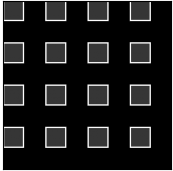
\includegraphics[width=1.5cm]{papers_src/BeyondGrids/figures/elasticities/scale/50.png}}
               & \raisebox{-.5\height}{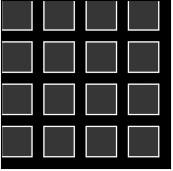
\includegraphics[width=1.5cm]{papers_src/BeyondGrids/figures/elasticities/scale/75.png}}
               & \raisebox{-.5\height}{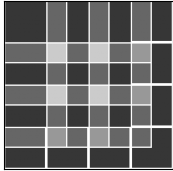
\includegraphics[width=1.5cm]{papers_src/BeyondGrids/figures/elasticities/scale/150.png}}
               & \raisebox{-.5\height}{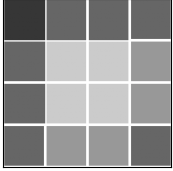
\includegraphics[width=1.5cm]{papers_src/BeyondGrids/figures/elasticities/scale/200.png}} \\[12pt]
        & 12.5\% & 25\% & 37.5\% & 50\% \\
        Position & \raisebox{-.5\height}{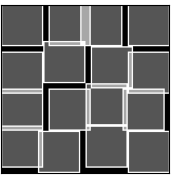
\includegraphics[width=1.5cm]{papers_src/BeyondGrids/figures/elasticities/position/12.5.png}}
                  & \raisebox{-.5\height}{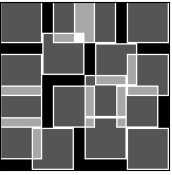
\includegraphics[width=1.5cm]{papers_src/BeyondGrids/figures/elasticities/position/25.png}}
                  & \raisebox{-.5\height}{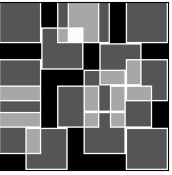
\includegraphics[width=1.5cm]{papers_src/BeyondGrids/figures/elasticities/position/37.5.png}}
                  & \raisebox{-.5\height}{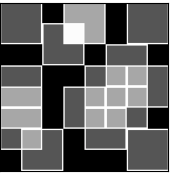
\includegraphics[width=1.5cm]{papers_src/BeyondGrids/figures/elasticities/position/50.png}} \\[12pt]
        & 20\% & 40\% & 60\% & 80\% \\
        Missing data & \raisebox{-.5\height}{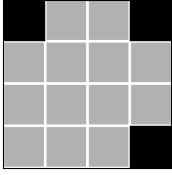
\includegraphics[width=1.5cm]{papers_src/BeyondGrids/figures/elasticities/dropout/20.png}}
                      & \raisebox{-.5\height}{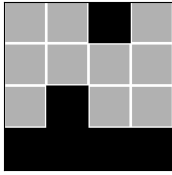
\includegraphics[width=1.5cm]{papers_src/BeyondGrids/figures/elasticities/dropout/40.png}}
                      & \raisebox{-.5\height}{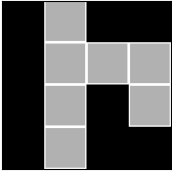
\includegraphics[width=1.5cm]{papers_src/BeyondGrids/figures/elasticities/dropout/60.png}}
                      & \raisebox{-.5\height}{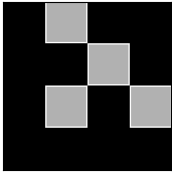
\includegraphics[width=1.5cm]{papers_src/BeyondGrids/figures/elasticities/dropout/80.png}} \\
    \end{tabular}
    \end{small}
    \caption[The three types of input elasticity evaluated in Beyond Grids]{\textbf{Elasticity perturbations.} Each row illustrates one type of perturbation applied to an example image at increasing intensity. \emph{Scale}: patches are sampled at sizes ranging from 50\% to 200\% of the native $16\times16$ size (undersampling introduces gaps while oversampling introduces overlap). \emph{Position}: patches are displaced from their grid positions by up to 50\% of the patch size (patch shake). \emph{Missing data}: an increasing fraction of patches is dropped from the input. Adapted from~\pubcite{pardyl2023grids}.}
    \label{fig:beyond-perturbations}
\end{figure}

The publication introduces the concept of \emph{input elasticity} as resilience to particular
forms of input data configurations that can occur in real-life applications. Three distinct types of elasticity are defined, each corresponding to a perturbation commonly encountered in embodied AI applications and illustrated in Figure~\ref{fig:beyond-perturbations}.

\paragraph{Scale elasticity.} This measures resilience when individual patches are sampled at a scale different from the native $16\times16$ pixel resolution. Each patch $p = (x, y, s)$ is characterised by the pixel coordinates of its top-left corner $(x, y)$ and a relative scale $s$. The patch covers a $16s \times 16s$ pixel region in the original image, which is then resampled to the standard $16\times16$ input size. A scale of $s = 2$ means the patch covers four times the usual area at half the resolution, $s = 0.5$ covers one quarter the area at twice the resolution, potentially leaving uncovered gaps between adjacent patches. This corresponds to the zoom ability of a camera.

\paragraph{Positional elasticity.} Also called \emph{patch shake}, this measures resilience when patch positions are displaced from the regular grid. The coordinates $(x, y)$ of each patch are independently perturbed by an offset drawn uniformly from $[-r \cdot q,\, r \cdot q]$, where $r$ is the patch size and $q$ is the shake magnitude as a fraction of the patch size. This simulates the non-grid-aligned sampling that arises whenever an image is captured at a position that does not correspond exactly to a discrete training configuration, e.g. due to imperfect camera alignment or agent drift in real space.

\paragraph{Missing-data elasticity.} This measures resilience when a fraction $d$ of patches are simply removed from the input, leaving the corresponding image regions unobserved. This is the most directly relevant perturbation for active visual exploration, where an agent has only observed a subset of the scene, or has lost parts of it due to, e.g., occlusion or communication failure.

The three perturbations are composed into a pipeline. For image $I$, an initial patch set $P$ (standard grid, $s=1$, no displacement) is processed by
\begin{equation}
    P' = \mathcal{E}_{\mathrm{miss}(d)} \circ \mathcal{E}_{\mathrm{pos}(q)} \circ \mathcal{E}_{\mathrm{scale}(s_1, s_2)}(P),
    \label{eq:elasticity-pipeline}
\end{equation}
where $\mathcal{E}_{\mathrm{scale}(s_1,s_2)}$ samples each patch's scale independently from $[s_1, s_2]$, $\mathcal{E}_{\mathrm{pos}(q)}$ shifts each patch's top-left corner by at most $q$ patch-widths in each direction, and $\mathcal{E}_{\mathrm{miss}(d)}$ removes a fraction $d$ of the patches at random. Elasticity is high if predictive performance on the perturbed set $P'$ remains close to that on the~original~$P$.

\subsection{ElasticViT}
\label{sec:beyond-elasticvit}

\begin{figure}[th]
    \centering
    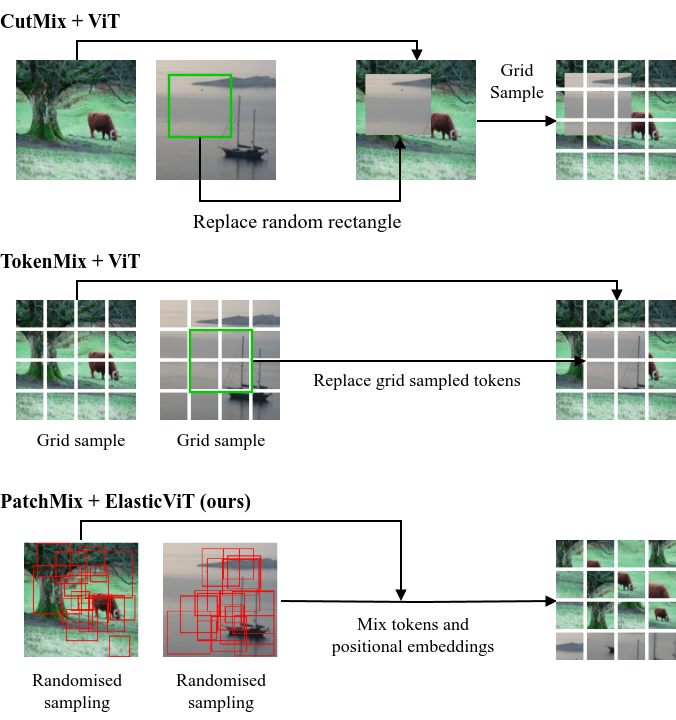
\includegraphics[width=.75\linewidth]{papers_src/BeyondGrids/figures/patchmix/patchmix.png}
    \caption[PatchMix augmentation compared to CutMix and TokenMix]{\textbf{PatchMix.} Unlike CutMix, which replaces a rectangular region of one image with another, PatchMix operates on individually sampled patches and mixes them at the token level. Unlike TokenMix, it does not assume grid-aligned patches, making it compatible with elastic sampling. Reproduced from~\pubcite{pardyl2023grids}.}
    \label{fig:patchmix}
\end{figure}

The modifications proposed in this publication to increase input elasticity are two-fold: a new continuous positional encoding that can represent patches at any position and scale, and a change to the training augmentation regime.

\paragraph{Continuous positional encoding.} As established in Section~\ref{sec:prelim-pos-enc}, both learnable and standard sinusoidal positional embeddings operate on a finite, discrete set of grid positions. Hence, they cannot represent a patch sampled at an arbitrary pixel-level position or at a variable scale. Our publication addresses this by replacing the learnable embeddings of standard ViT with a deterministic \emph{four-dimensional} sine-cosine encoding. Each patch $p$ is characterised by the pixel coordinates of its upper-left corner $(x, y)$ and its relative scale $s$ (where $s = 1$ corresponds to the native $16\times16$ patch size). The lower-right corner of the patch is then at $(x + 16s,\, y + 16s)$, and the full spatial extent of $p$ is described by the four scalar values $(x,\, y,\, x+16s,\, y+16s)$. Each of these four values is encoded independently with a 1D sine-cosine encoding (Equation~\ref{eq:sincos-enc}), and the resulting vectors are concatenated to form the patch's positional~embedding:
\begin{equation}
    \mathrm{PE}(p) = \bigl[\mathrm{pe}(x)\;\|\;\mathrm{pe}(y)\;\|\;\mathrm{pe}(x+16s)\;\|\;\mathrm{pe}(y+16s)\bigr],
    \label{eq:pos-enc}
\end{equation}
where $\mathrm{pe}(\cdot)$ is the 1D sine-cosine encoding and $\|$ denotes vector concatenation. Because this function is defined over the reals, it generalises without modification to any position-scale combination at inference, including configurations never seen during training. The ViT input is also modified accordingly. Instead of a full rasterised image, the model receives a list of cropped patches together with their corresponding coordinate tuples, which are fed into the positional encoding rather than looked up in a table.

\paragraph{Elastic training augmentations.} The baseline training regime follows DeiT~III~\cite{touvron2022deitiii}. To this, the publication adds the elasticity functions as augmentations during training. Patch sizes are drawn uniformly between $16\times16$ and $48\times48$ pixels, resampled to the $16\times16$ token size, and patch positions are sampled uniformly throughout the image. This forces the model to generalise across a wide distribution of patch configurations, rather than overfitting to the regular grid it would otherwise always see.

\paragraph{PatchMix augmentation.} The standard CutMix augmentation, which mixes two images by replacing a rectangular region of one image with the corresponding region from another, is incompatible with variable-scale patch sampling. The mixing ratios used to blend the class labels assume a fixed spatial layout that no longer holds when patches can overlap or leave gaps. The publication introduces PatchMix, an alternative that performs mixing at the level of individual \emph{patches after sampling}. Patches from two images are randomly interleaved in the token sequence, and the label blending ratio is computed from the actual proportion of patches drawn from each image. Unlike the previously proposed TokenMix~\cite{liu2022tokenmix}, PatchMix does not assume grid-aligned sampling and is therefore fully compatible with the elastic augmentation regime (see Figure~\ref{fig:patchmix}).

\subsection{Experimental results}
\label{sec:beyond-results}


\paragraph{Elasticity evaluation.} Figure~\ref{fig:beyond-elasticity} shows the three single-perturbation elasticity curves, comparing our ElasticViT against ViT, MAE, Swin-B, and PVT-v2-B5, all of comparable size and trained on ImageNet-1k.

\begin{figure}[t]
\begin{center}
\begin{small}
\begin{subfigure}[b]{0.32\textwidth}
\begin{tikzpicture}
\tikzstyle{every node}=[font=\scriptsize]
\begin{axis}[
    title={Patch scale},
    xlabel={Scale},
    ylabel={Accuracy (\%)},
    xtick={-8,0,8},
    xticklabels={0.5,1,2},
    xmin=-8,
    xmax=8,
    ymin=55,
    ymajorgrids=true,
    grid style=dashed,
    scale only axis,
    height=3cm,
    width=.75\linewidth,
    legend to name=beyond-elasticity-legend,
    legend style={/tikz/every even column/.append style={column sep=0.1cm},font=\tiny},
    legend cell align={left},
    legend columns=5
]
    \addplot[color=red]
    coordinates {
    (-8,74.200)(-7,76.928)(-6,79.364)(-5,81.156)(-4,82.268)(-3,82.760)(-2, 83.206)(-1, 83.264)(0,83.800)(1, 83.358)(2, 82.936)(3, 82.142)(4, 82.138)(5, 79.860)(6, 78.000)(7, 76.148)(8, 73.790)
    };
    \addlegendentry{ViT}
    \addplot[color=darkorange25512714]
    coordinates {
    (-8,73.1)(-7,75.5)(-6,77.4)(-5,79.3)(-4,80.7)(-3,81.8)(-2,82.7)(-1,83.2)(0,83.6)(1,83.4)(2,82.8)(3,81.7)(4,80.4)(5,78.8)(6,76.2)(7,72.8)(8,67.7)
    };
    \addlegendentry{MAE}
    \addplot[color=forestgreen4416044]
    coordinates {
    (-8,44.4)(-7,52.0)(-6,58.7)(-5,66.3)(-4,71.7)(-3,75.5)(-2,79.3)(-1,82.0)(0,83.8)(1,82.0)(2,80.8)(3,79.0)(4,76.8)(5,74.8)(6,72.0)(7,68.4)(8,62.97)
    };
    \addlegendentry{PVT}
    \addplot[color=gray]
    coordinates {
    (-8,54.3)(-7,63.5)(-6,68.2)(-5,74.1)(-4,78.0)(-3,80.1)(-2,81.8)(-1,82.7)(0,83.5)(1,82.2)(2,82.0)(3,80.8)(4,78.2)(5,78.3)(6,76.1)(7,72.8)(8,68.4)
    };
    \addlegendentry{Swin}
    \addplot[color=steelblue31119180, very thick]
    coordinates {
    (-8,80.552)(-7,81.186)(-6,81.422)(-5,81.684)(-4,81.896)(-3,81.974)(-2, 82.016)(-1, 81.944)(0,82.036)(1, 81.780)(2, 81.240)(3, 80.790)(4, 79.742)(5, 79.594)(6, 78.898)(7, 78.244)(8, 77.504)
    };
    \addlegendentry{ElasticViT (ours)}
\end{axis}
\end{tikzpicture}
\caption{}
\label{fig:beyond-zoom}
\end{subfigure}
\hfill
\begin{subfigure}[b]{0.32\textwidth}
\begin{tikzpicture}
\tikzstyle{every node}=[font=\scriptsize]
\begin{axis}[
    title={Missing data},
    xlabel={Patches dropped (\%)},
    xtick={1,3,5,7,9},
    xticklabels={0,20,40,60,80},
    xmin=1,
    xmax=9,
    ymin=58,
    ymajorgrids=true,
    grid style=dashed,
    scale only axis,
    height=3cm,
    width=.75\linewidth,
    legend cell align={left}
]
    \addplot[color=red]
    coordinates {
    (1,83.800)(2,83.316)(3,82.740)(4,81.852)(5,80.752)(6,79.042)(7,75.826)(8,70.154)(9,58.416)
    };
    \addplot[color=darkorange25512714]
    coordinates {
    (1,83.638)(2,83.394)(3,83.120)(4,82.540)(5,81.744)(6,80.392)(7,78.220)(8,74.304)(9,66.862)
    };
    \addplot[color=forestgreen4416044]
    coordinates {
    (1,83.792)(2,82.696)(3,80.814)(4,78.500)(5,75.208)(6,70.974)(7,65.408)(8,58.762)(9,50.032)
    };
    \addplot[color=gray]
    coordinates {
    (1,83.482)(2,83.038)(3,82.342)(4,81.556)(5,80.220)(6,78.194)(7,75.634)(8,71.044)(9,62.350)
    };
    \addplot[color=steelblue31119180, very thick]
    coordinates {
    (1,82.036)(2,81.65)(3,81.276)(4,80.738)(5,80.046)(6,78.904)(7,77.328)(8,74.620)(9,68.582)
    };
\end{axis}
\end{tikzpicture}
\caption{}
\label{fig:beyond-dropout}
\end{subfigure}
\hfill
\begin{subfigure}[b]{0.32\textwidth}
\begin{tikzpicture}
\tikzstyle{every node}=[font=\scriptsize]
\begin{axis}[
    title={Patch position},
    xlabel={Patch shake (\%)},
    xtick={1,3,5,7,9},
    xticklabels={0,12.5,25,37.5,50},
    xmin=1,
    xmax=9,
    ymin=77,
    ymajorgrids=true,
    grid style=dashed,
    scale only axis,
    height=3cm,
    width=.75\linewidth,
    legend cell align={left}
]
    \addplot[color=red]
    coordinates {
    (1,83.800)(2,83.728)(3,83.524)(4,83.222)(5,82.954)(6,82.504)(7,81.964)(8,81.532)(9,80.838)
    };
    \addplot[color=darkorange25512714]
    coordinates {
    (1,83.638)(2,83.654)(3,83.534)(4,83.350)(5,83.048)(6,82.798)(7,82.494)(8,82.124)(9,81.768)
    };
    \addplot[color=forestgreen4416044]
    coordinates {
    (1,83.796)(2,82.926)(3,81.732)(4,80.110)(5,78.252)(6,76.402)(7,74.196)(8,71.718)(9,69.016)
    };
    \addplot[color=gray]
    coordinates {
    (1,83.482)(2,83.286)(3,83.022)(4,82.750)(5,82.206)(6,81.688)(7,81.078)(8,80.340)(9,79.446)
    };
    \addplot[color=steelblue31119180, very thick]
    coordinates {
    (1,82.036)(2,81.946)(3,82.012)(4,81.950)(5,81.830)(6,81.738)(7,81.704)(8,81.496)(9,81.294)
    };
\end{axis}
\end{tikzpicture}
\caption{}
\label{fig:beyond-shake}
\end{subfigure}
\par\medskip
\ref{beyond-elasticity-legend}
\end{small}
\end{center}
\caption[Elasticity curves for individual perturbations on ImageNet-1k]{\textbf{Elasticity under isolated perturbations} (ImageNet-1k top-1 accuracy). \textbf{(a)}~Scale elasticity: all baselines degrade sharply when patches deviate from scale~1, while our ElasticViT maintains near-constant accuracy across the measured spectrum and outperforms all baselines at extreme scales. \textbf{(b)}~Missing-data elasticity: ElasticViT surpasses MAE from 70\% dropout onward, despite never being trained with patch dropout. \textbf{(c)}~Positional elasticity: ElasticViT is nearly immune to patch shake and outperforms all but MAE at the largest perturbations. Adapted from~\pubcite{pardyl2023grids}.}
\label{fig:beyond-elasticity}
\end{figure}

Under standard conditions (centre of each curve, scale~1, no dropout, no shake), ElasticViT trails ViT by $\approx$1.8 pp. However, as perturbation intensity increases, the gap reverses and widens considerably. At 2$\times$ scale, ElasticViT outperforms ViT by $\approx$3.7 pp and at 80\% missing data, it outperforms MAE (the strongest baseline in that regime) by $\approx$1.7 pp. When perturbations are combined, the advantage grows even further: under simultaneous scale and position perturbation at their maxima, ElasticViT leads ViT by nearly 20 percentage points. Standard ViTs, in effect, overfit to the specific grid configuration used during training, while our ElasticViT trades a small amount of peak accuracy on that configuration for robustness across the whole spectrum of input perturbations.

\paragraph{Adaptive sampling.} To test the usefulness of ElasticViT for visual exploration problems, the publication proposes two simple, non-learnable baseline sampling strategies: CENTRAL (retina-like sampling) and EDGE (edge-detection-based sampling), illustrated in Figure~\ref{fig:beyond-edge-vis}. Figure~\ref{fig:beyond-adaptive} shows their effect on accuracy as a function of the number of input patches.

\begin{figure}[t]
\centering
\begin{tikzpicture}[node distance=0.3cm, auto]
\tikzstyle{pict} = [inner xsep=4px]
\tikzstyle{arrow} = [thick,->,>=latex]
\node [pict] (input) {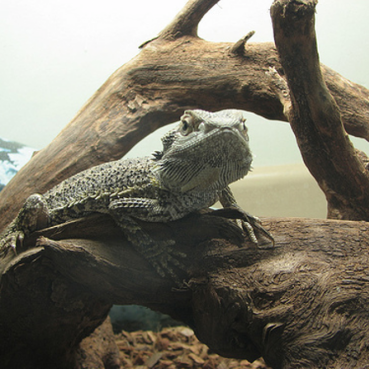
\includegraphics[width=2cm]{papers_src/BeyondGrids/figures/edge/edges1.png}};
\node [above=2pt of input, font=\scriptsize\scshape] {Input};
\node [pict, right=1cm of input] (central) {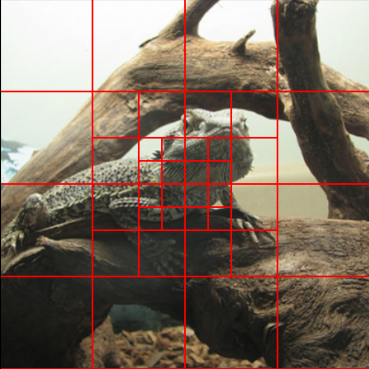
\includegraphics[width=2cm]{papers_src/BeyondGrids/figures/edge/central.png}};
\node [above=2pt of central, font=\scriptsize\scshape] {CENTRAL};
\node [pict, below=0.5cm of central] (edge) {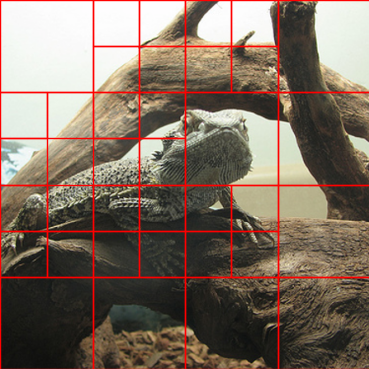
\includegraphics[width=2cm]{papers_src/BeyondGrids/figures/edge/edges3.png}};
\node [above=2pt of edge, font=\scriptsize\scshape] {EDGE};
\draw [arrow] (input) -- (central);
\draw [arrow] (input) -- (edge);
\end{tikzpicture}
\caption[CENTRAL and EDGE adaptive patch sampling strategies]{\textbf{Adaptive sampling strategies.} CENTRAL iteratively subdivides patches closest to the image centre into four smaller ones, producing higher resolution in the foveal region (analogous to retinal sampling). EDGE uses a Canny edge detector~\cite{canny1986computational} to concentrate small patches on high-frequency regions. Reproduced from~\pubcite{pardyl2023grids}.}
\label{fig:beyond-edge-vis}
\end{figure}

\begin{figure}[t]
\begin{center}
\begin{small}
\begin{tikzpicture}
\tikzstyle{every node}=[font=\scriptsize]
\begin{axis}[
    title={Sampling strategies},
    xlabel={No.\ input patches (log scale)},
    ylabel={Accuracy (\%)},
    xtick={16,64,196,784},
    xmin=16,
    xmax=784,
    ymin=38,
    ymax=87,
    ymajorgrids=true,
    grid style=dashed,
    scale only axis,
    height=3.5cm,
    width=.75\linewidth,
    legend pos=south east,
    legend cell align={left},
    xmode=log,
    log ticks with fixed point,
]
    \addplot[color=red, dashed]
    coordinates {
    (16,19.8)(25,44.9)(36,60.9)(49,73.6)(64,75.9)(81,79.0)(100,79.8)(121,81.0)(144,81.8)(169,82.6)(196,83.8)(225,83.1)(256,83.3)(324,82.7)(361,82.5)(441,81.8)(529,80.5)(625,79.7)(784,77.4)
    };
    \addlegendentry{ViT, grid}
    \addplot[color=red]
    coordinates {
    (16,19.8)(24,45.5)(28,62.0)(40,66.9)(49,73.6)(54,75.1)(76,79.4)(124,82.5)(196,83.8)(208,83.5)(244,83.5)(302,81.6)(388,80.4)(496,80.0)(628,78.6)(784,77.4)
    };
    \addlegendentry{ViT, central}
    \addplot[color=steelblue31119180, dashed]
    coordinates {
    (16,40.6)(25,58.1)(36,67.4)(49,73.2)(64,75.4)(81,77.8)(100,78.5)(121,79.7)(144,80.6)(169,81.3)(196,82.0)(225,82.3)(256,82.4)(324,82.8)(361,82.8)(441,83.0)(529,83.1)(625,83.2)(784,83.1)
    };
    \addlegendentry{ElasticViT (ours), grid}
    \addplot[color=steelblue31119180]
    coordinates {
    (16,40.6)(24,59.8)(28,65.1)(40,70.3)(49,73.2)(54,74.8)(76,78.5)(124,80.9)(196,82.0)(208,82.2)(244,82.5)(302,82.7)(388,82.8)(496,82.9)(628,83.1)(784,83.1)
    };
    \addlegendentry{ElasticViT (ours), central}
    \addplot[color=forestgreen4416044]
    coordinates {
    (16,52.6)(25,64.5)(36,70.4)(49,74.6)(64,77.1)(81,78.6)(100,79.7)(121,80.2)(144,80.9)(169,81.2)(196,81.4)(225,81.6)(256,81.9)(324,81.9)(361,82.1)(441,82.1)(529,82.3)(625,82.4)(784,83.1)
    };
    \addlegendentry{ElasticViT (ours), edge}
\end{axis}
\end{tikzpicture}
\end{small}
\end{center}
\caption[Accuracy vs.\ patch count for adaptive sampling strategies]{\textbf{Adaptive sampling strategies vs.\ standard grid} (ImageNet-1k accuracy). At 16 patches, ElasticViT with EDGE sampling achieves 52.6\%, versus 40.6\% for ElasticViT on a grid (+12 pp) and 19.8\% for ViT on a grid (+32 pp). The rigid ViT does not benefit from CENTRAL sampling because it cannot interpret non-grid patch positions. Adapted from~\pubcite{pardyl2023grids}.}
\label{fig:beyond-adaptive}
\end{figure}

At 16 input patches (a severely limited observation budget directly analogous to the earliest stages of active visual exploration), EDGE sampling with ElasticViT achieves 52.6\%, compared to 40.6\% for the same model on a standard grid and only 19.8\% for rigid ViT on a grid. The rigid ViT does not benefit from CENTRAL sampling in this low-patch regime, because its learnable positional embeddings cannot generalise to the non-grid-aligned positions CENTRAL produces. ElasticViT, by contrast, handles these positions natively through its continuous positional encoding.

Further experimental results are presented in the original paper~\pubcite{pardyl2023grids}.

\subsection{Contributions}
\label{sec:contributions-beyond}

The publication ``Beyond Grids: Exploring Elastic Input Sampling for Vision Transformers''~\pubcite{pardyl2023grids} makes the following contributions to the field:

\begin{itemize}
    \item It formalises the notion of \emph{input elasticity} for vision transformers across three dimensions (scale, position, and missing data) and introduces an evaluation protocol that enables direct comparison of models on each dimension and demonstrates empirically that standard ViTs are fragile under these perturbations, with accuracy dropping sharply even for moderate scale or dropout levels.
    \item It proposes ElasticViT, combining a continuous four-dimensional positional encoding (replacing learnable embeddings) with elastic training augmentations and the new PatchMix augmentation. ElasticViT achieves near-constant accuracy across the full range of scale and position perturbations, and surpasses MAE on missing-data resilience despite never being trained with patch dropout.
    \item It introduces the CENTRAL and EDGE adaptive patch sampling baseline strategies, and shows that these strategies provide large accuracy gains at low patch counts (up to $+32$ pp over rigid ViT at 16 patches) \emph{only} when combined with an elastic backbone.
\end{itemize}

The robustness of ElasticViT across the three evaluated perturbation types, together with its gains from adaptive sampling at low patch counts, confirms Hypothesis~\ref{hyp:beyond} within the evaluated settings.

I was the first and primary author of this paper. I contributed to the conception of the idea and designed the training regime, positional encoding, and augmentation strategy. I carried out the majority of the experimental design and implementation, conducted the majority of the experiments presented in the paper, and contributed significantly to writing the manuscript. I also presented the research at the IEEE/CVF Winter Conference on Applications of Computer Vision (WACV) 2025 in Tucson, Arizona, USA. The code and data are available on my GitHub at \url{https://github.com/apardyl/beyondgrids}.
